\documentclass[]{article}
\usepackage{circuitikz}
\usepackage{graphicx}
\usepackage{listings}
\usepackage{xcolor}
\definecolor{codegreen}{HTML}{859900}
\definecolor{codegray}{HTML}{839496}
\definecolor{codepurple}{HTML}{6C71C4}
\definecolor{codemagenta}{HTML}{d33682}
\definecolor{backcolour}{HTML}{FDF6E3}
\definecolor{fontcolor}{HTML}{002B36}
\lstdefinestyle{mystyle}{
	basicstyle=\color{fontcolor},
	backgroundcolor=\color{backcolour},   
	commentstyle=\color{codegreen},
	keywordstyle=\color{codemagenta},
	numberstyle=\tiny\color{codegray},
	stringstyle=\color{codepurple},
	breakatwhitespace=false,         
	breaklines=true,                 
	captionpos=b,                    
	keepspaces=true,                 
	numbers=left,                    
	numbersep=5pt,                  
	showspaces=false,                
	showstringspaces=false,
	showtabs=false,                  
	tabsize=4
}
\lstset{style=mystyle}
\title{Lab 7\\Displays}
\author{Keaton Clark}

\begin{document}
\maketitle
\section*{Circuit}
I did not purchase the kit as I have *most* of the parts required for the class. One of the parts I did not have was the button matrix so I needed to build one myself. Here is the schematic.
\begin{center}
\begin{circuitikz}
	\draw (1,4) to
		[short,-](1,0) to
		[short, l={$D_{23}$},o-](1,0)
	;
	\draw (2,4) to
		[short,-](2,0) to
		[short, l={$D_{25}$},o-](2,0)
	;
	\draw (3,4) to
		[short,-](3,0) to
		[short, l={$D_{27}$},o-](3,0)
	;
	\draw (3,4) to
		[short, -](0,4) to
		[short, l={$D_{22}$},o-](0,4)
	;
	\draw (3,3) to
		[short, -](0,3) to
		[short, l={$D_{24}$},o-](0,3)
	;
	\draw (3,2) to
		[short, -](0,2) to
		[short, l={$D_{26}$},o-](0,2)
	;
	\draw (3,1) to
		[short, -](0,1) to
		[short, l={$D_{28}$},o-](0,1)
	;
	\draw (1,.5) to
		[push button](.5,1)
	;
	\draw (1,1.5) to
		[push button](.5,2)
	;
	\draw (1,2.5) to
		[push button](.5,3)
	;
	\draw (1,3.5) to
		[push button](.5,4)
	;
	\draw (2,.5) to
		[push button](1.5,1)
	;
	\draw (2,1.5) to
		[push button](1.5,2)
	;
	\draw (2,2.5) to
		[push button](1.5,3)
	;
	\draw (2,3.5) to
		[push button](1.5,4)
	;
	\draw (3,.5) to
		[push button](2.5,1)
	;
	\draw (3,1.5) to
		[push button](2.5,2)
	;
	\draw (3,2.5) to
		[push button](2.5,3)
	;
	\draw (3,3.5) to
		[push button](2.5,4)
	;
\end{circuitikz}\\
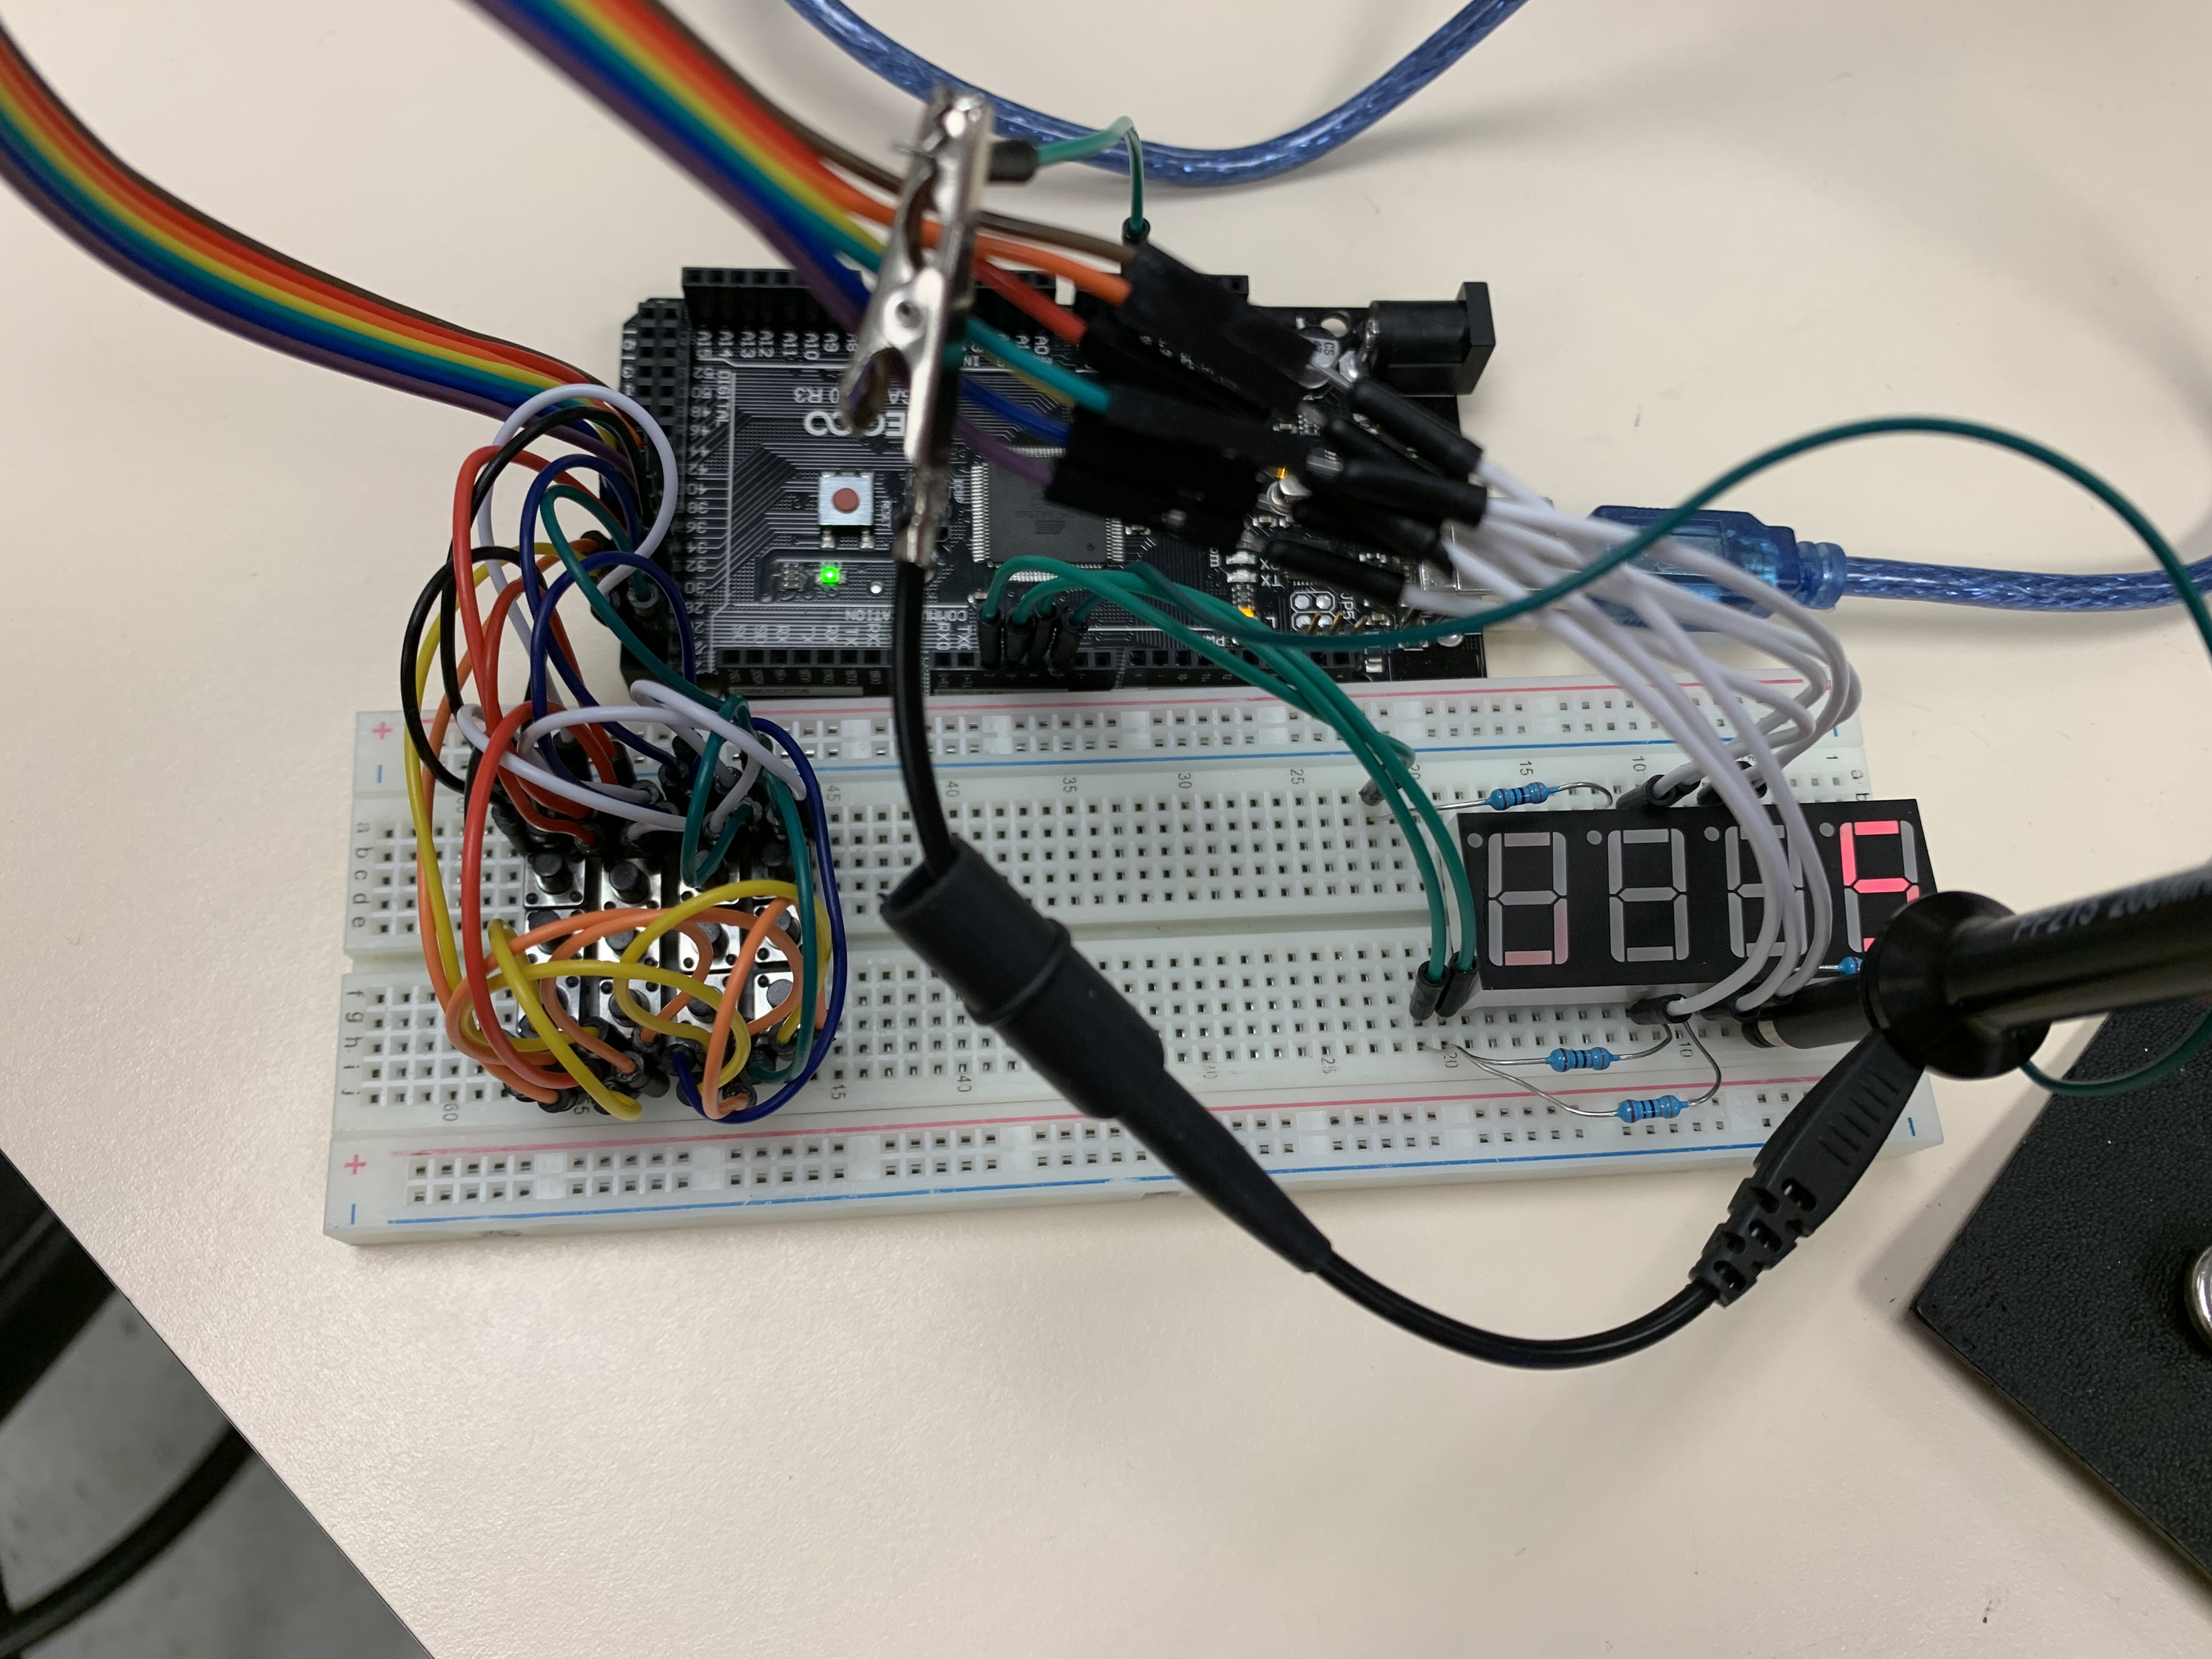
\includegraphics[width=\textwidth]{ ./images/1.jpg }
\end{center}
\pagebreak
\section*{Code}
The important logical portion of main.c, everything above is just initializing the button matrix and the 7 segment display. Looking back at my code I see it actually gets stuck at the first while loop (updating the display the whole time) until a button is pressed then it loops backwards from i=3, only decrementing when a key is pressed and write the value of the keypress to the ith eleement of a 4 element char array. Write the char array to the display and then get stuck at the while loop updating the display until the key is unpressed and then another key is later pressed.\\
Once it reads four chars it breaks out of the loop and goes into a psuedo delay loop updating the whole time so that we can see the keys we just input. Then clear the char array, write the clear array to the display, update, and do it all again.
\lstinputlisting[firstline=49,lastline=68,firstnumber=49]{ ../src/main.c }
\pagebreak
The matrix code is pretty simple. In the init set all rows to outputs and pull them high, and set all the columns to inputs and activate their internal pullups. Then to read a certain button on the matrix set its corresponding row to low and read the value on its corresponding column.
\lstinputlisting[]{ ../src/matrix.c }
\pagebreak
The seven segment code is a similar idea as the matrix. Set all segment and digit pins as outputs and write all of the digit pins high. Then when you want to write to a digit, pull that one low and use the lookup table to receive an array with each element being the state of the segment in the corresponding number you used in the table. Then loop through the segments and write to them the state that the table tells you to. In order to generate this table I just used trial and error writing digits to the display.
\lstinputlisting[]{ ../src/sevenseg.c }
\pagebreak
\section*{Question}
\begin{itemize}
	\item One of the leads of the seven segment display (I believe this is one of the segment leads) is showing a square wave. This is because the Arduino cannot write to each digit at all times so it cycles through them and there is a small delay in between each digit, although unseen to the naked eye. This segment seems to be turned on for each of the digits, otherwise there would be a corresponding gap in the square wave.
		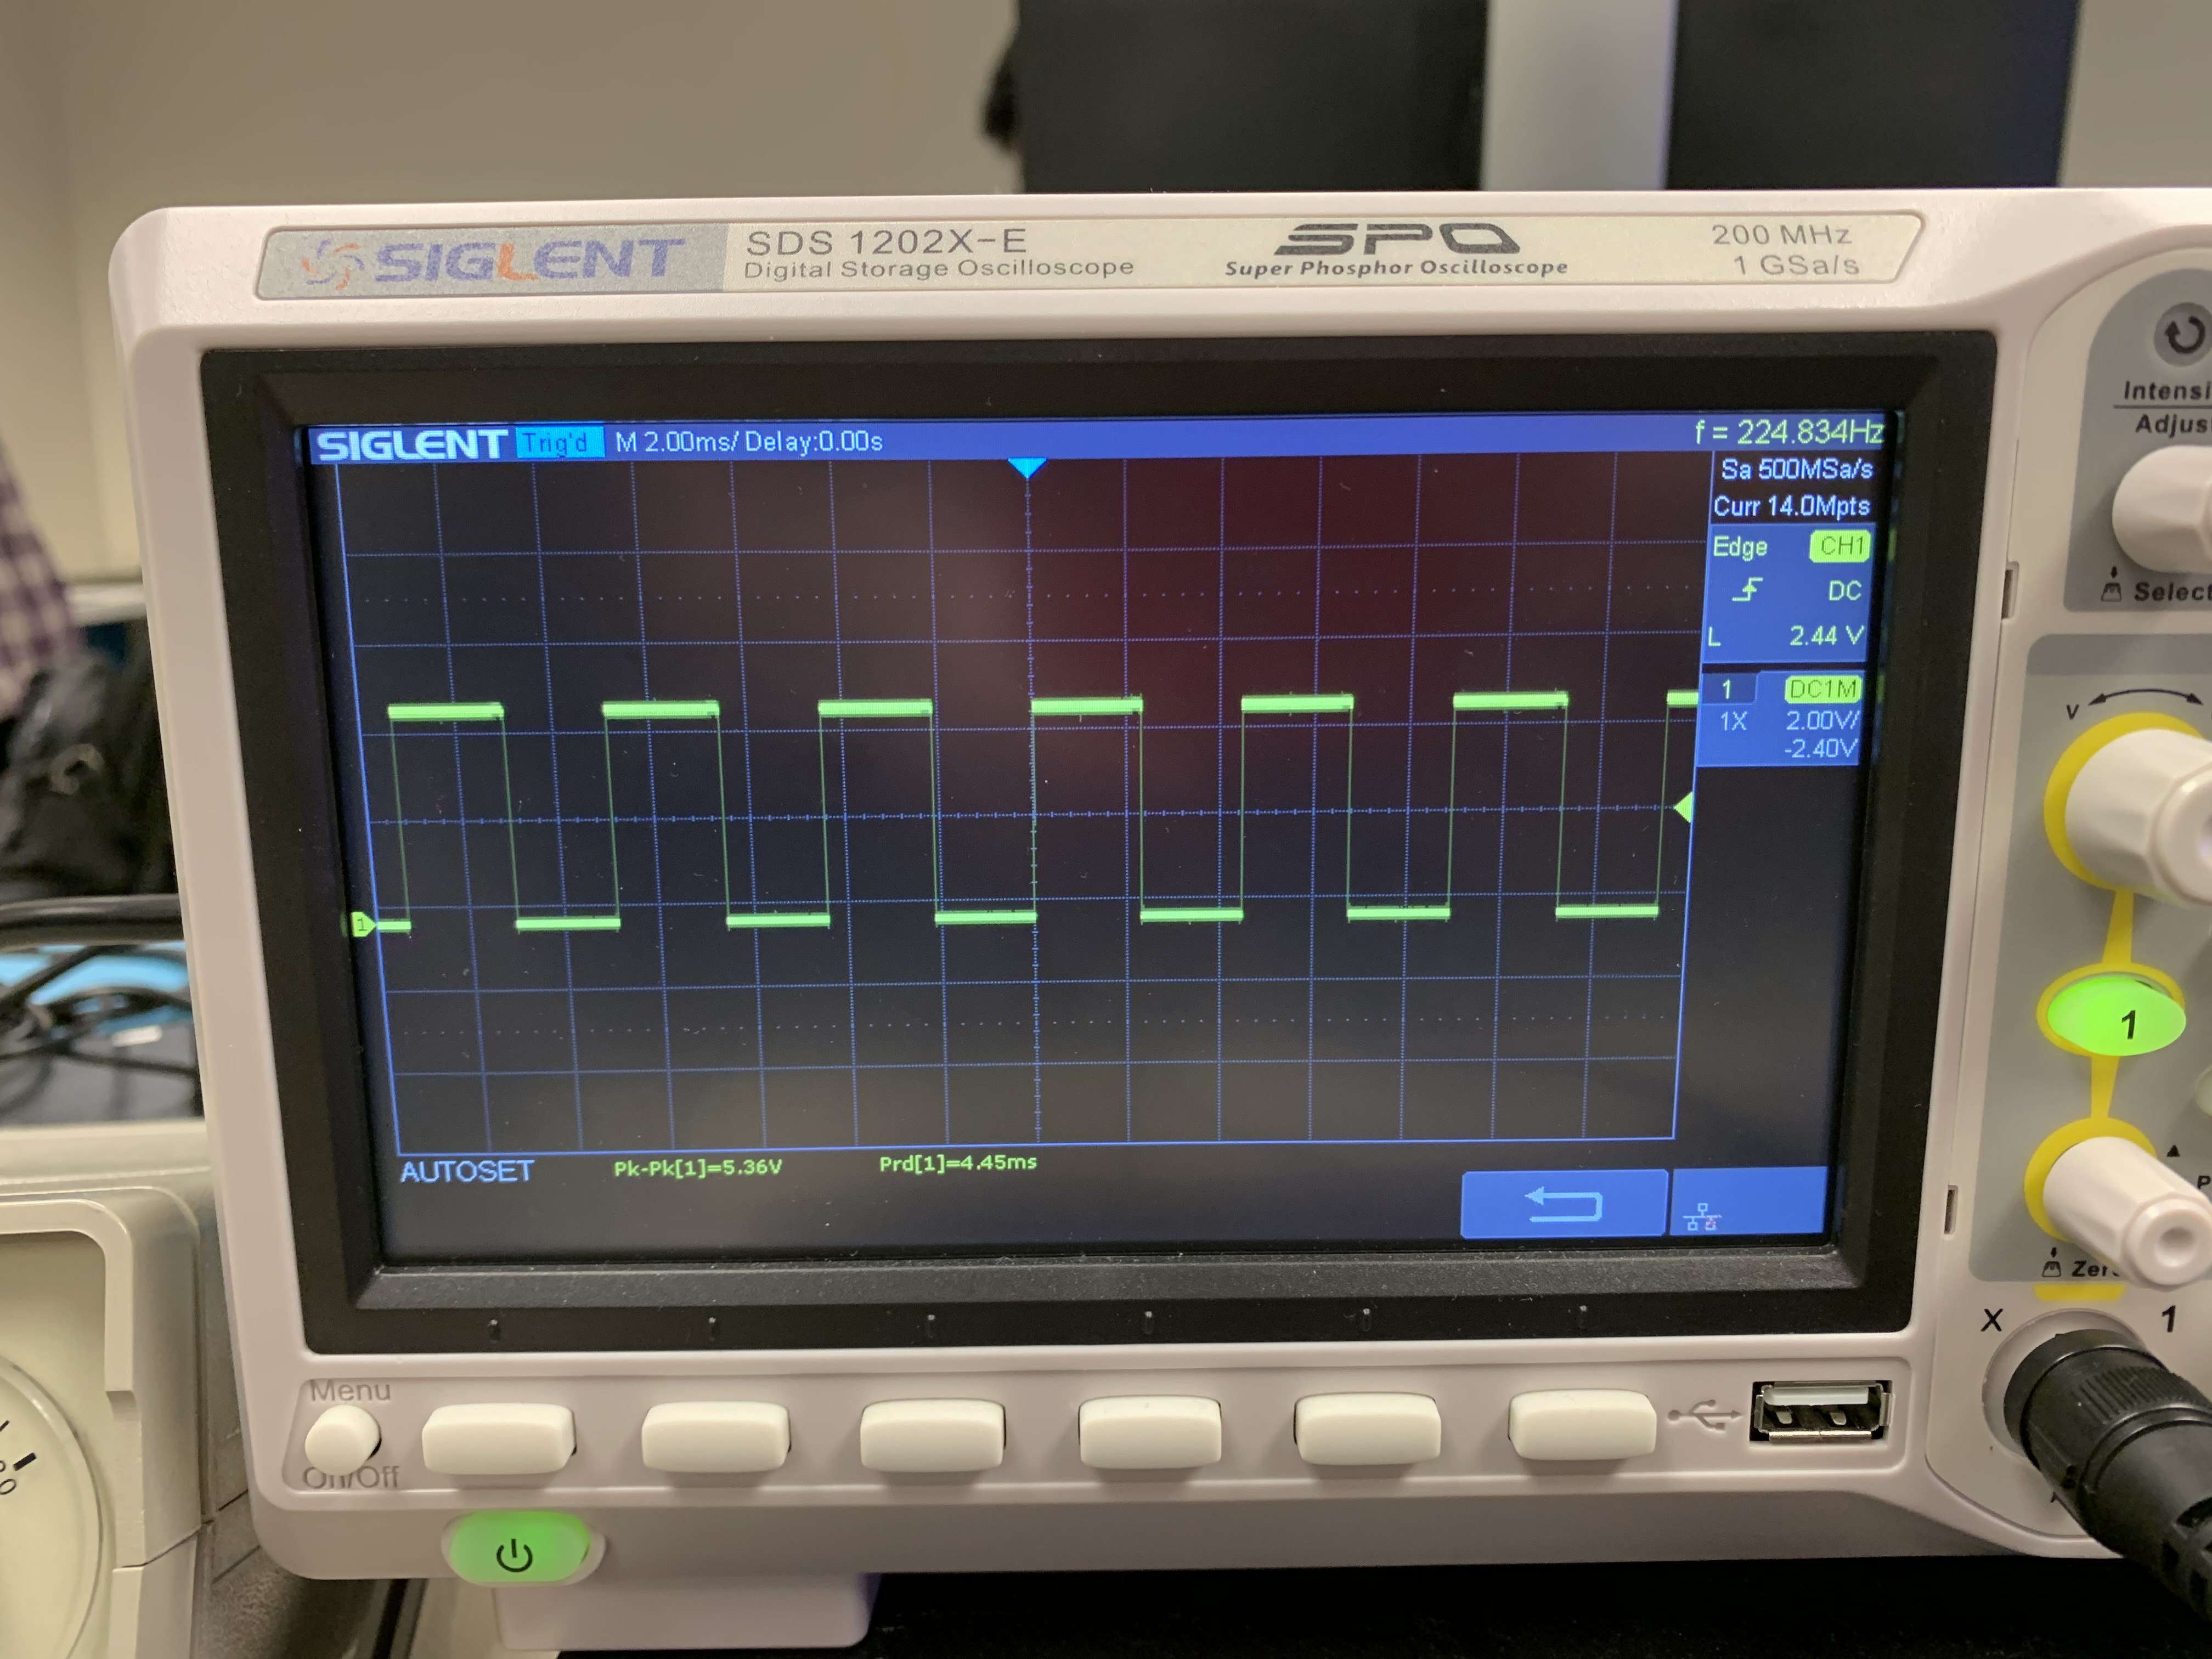
\includegraphics[width=\textwidth]{ ./images/3.jpg }
\end{itemize}
\end{document}
